\documentclass[a4paper,12pt]{article} 

%%% Работа с русским языком
\usepackage{cmap}                           % поиск в PDF
\usepackage{mathtext} 			 	       % русские буквы в формулах
\usepackage[T2A]{fontenc}               % кодировка
\usepackage[utf8]{inputenc}              % кодировка исходного текста
\usepackage[english,russian]{babel}  % локализация и переносы
\usepackage[left=2cm,right=2cm,
    top=2cm,bottom=3cm,bindingoffset=0cm]{geometry}
\usepackage{wrapfig}
\usepackage{gensymb}
\usepackage{textcomp}
\usepackage{multirow}
\usepackage{amsmath,amsfonts,amssymb,amsthm,mathtools} % AMS
\usepackage{euscript}	 % Шрифт Евклид
\usepackage{mathrsfs} % Красивый матшрифт
\usepackage{graphicx}%Вставка картинок правильная
\usepackage{float}%"Плавающие" картинки
\usepackage{wrapfig}%Обтекание фигур (таблиц, картинок и прочего)
\title{Лабораторная работа 3.7.1 

Скин-эффект в полом цилиндре}
\author{Кагарманов Радмир Б01-106}
\date{7 октября 2022 г.}

\begin{document}
\maketitle
\thispagestyle{empty}
\newpage
\setcounter{page}{1}

\paragraph{Цель работы:}исследование проникновения переменного магнитного поля в медный полый цилиндр.

\paragraph{В работе используется:}генератор звуковой частоты, соленоид, намотанный на полый цилиндрический каркас из диэлектрика, медный экран в виде трубки, измерительная катушка, амперметр, вольтметр, осциоллограф.

\paragraph{Теоретические сведения\\}
Связь между $H_0$ и $H_1$:
\begin{equation}
    H_1=\frac{H_0}{ch(\alpha h) + \frac{1}{2}\alpha a sh(\alpha h)},
\end{equation}
где $a=r$ - расстояние до оси системы, $h$ - толщина стенки цилиндра.\par

Рассмотрим предельные случаи:\par
1. При малых частотах толщина скин-слоя превосходит толщину цилиндра $\delta \gg h$. Тогда $|\alpha h| \approx 1,~ sh \alpha h \approx \alpha h$ и 
\begin{equation}
    H_1 \approx \frac{H_0}{1 + i\frac{ah}{\delta^2}}.
\end{equation}
Заметим, что величина $ah/\delta^2$ в общей случае не мала, поскольку при $h\ll a$ возможна ситуация $h\ll \delta \ll a$. Отношение модулей амплитуд здесь будет равно
\begin{equation}
    \frac{|H_1|}{|H_0|} = \frac{1}{\sqrt{1 + (\frac{ah}{\delta^2})^2}}=\frac{1}{\sqrt{1 + \frac{1}{4}(ah\sigma \mu_0 \omega)^2}}.
\end{equation}
При этом колебания $H_1$ отстают по фозе от $H_0$ на угол $\psi$, определяемый равенством $tg~ \psi = \frac{ah}{\delta^2}$.\par
2. При достаточно больших частотах толщина скин-слоя станет меньше толщины стенки: $\delta \ll h$. Тогда $|ah|\gg 1$, а также $sh (ah)\approx ch(ah)\approx \frac{1}{2}e^{\alpha h}$. Выражение (1) переходит в 
\begin{equation}
    \frac{H_1}{H_0}=\frac{4}{\alpha a}e^{-\alpha h}=\frac{2\sqrt{2} \delta}{a}e^{-\frac{h}{\delta}}e^{-i(\frac{\pi}{4}+\frac{h}{\delta})}.
\end{equation}
Поле внутри цилиндра по модулю в $\frac{2\sqrt{2} \delta}{a}e^{-\frac{h}{\delta}}$ раз меньше, чем снаружи, и запаздывает по фазе на
\begin{equation}
    \psi = \frac{\pi}{4} + \frac{h}{\delta}=\frac{\pi}{4}+h\sqrt{\frac{\omega \sigma \mu_0}{2}}.
\end{equation}\newpage

\begin{figure}[!h]
\centering
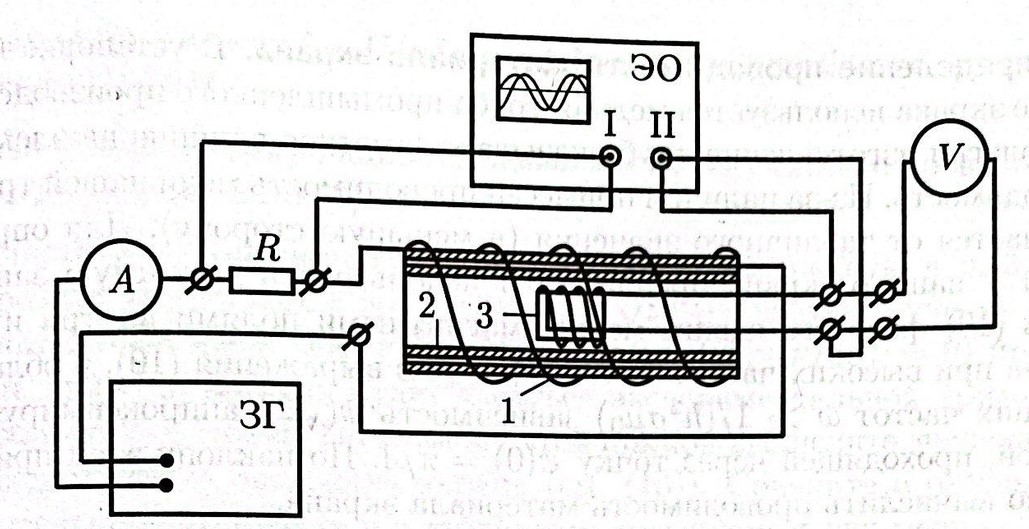
\includegraphics[width=0.9\linewidth]{установка.jpg}
\caption{Экспериментальная установка}
\label{fig:mpr}
\end{figure}

Схема экспериментальной установки для исследования проникновения переменного магнитного поля в медный полый цилиндр изображена на рис.1. Переменное поле создаётся с помощью соленоида, намотанного на полый цилиндрический каркас 1 из поливинилхлорида, который подключается к генератору звуковой частоты. Внутри соленоида расположен медный цилиндрический экран 2. Для измерения магнитного поля внутри экрана используется измерительная катушка 3. Действующее значение переменного тока в цепи соленоида измеряется амперметром $A$, а действующее значение напряжения на измерительной катушке измеряет вольтметр $V$. Для измерения сдвига фаз между током в цепи соленоида и напряжением на измерительной катушке используется двухканальный осциоллограф. На вход одного канала подаётся напряжение с резистора $R$, которое пропорционально току, а на вход второго канала - напряжение с измерительной катушки.
\paragraph{Измерение отношения амплитуд магнитного поля внутри и вне экрана.\\}
С помощью вольтметра $V$ измеряется действующее значение ЭДС индукции, которая возникает в измерительной катушке, находящейся в переменном магнитном поле $H_1 e^{i\omega t}$. Комплексная амплитуда ЭДС индукции в измерительной катушке равна
\begin{center}
    $U=-SN\frac{dB_{1}(t)}{dt}=-i\omega \mu_0 SNH_1 e^{i\omega t}$,
\end{center}
где $SN$ - произведение площади витка на число витков измерительной катушки. Показания вольтметра, измеряющего это напряжение:
\begin{center}
    $U=\frac{SN\omega}{\sqrt{2}}\mu_0 |H_1|$.
\end{center}
Видно, что модуль амплитуды магнитного поля внутри экрана $|H_1|$ пропорционален $U$ и обратно пропорционален частоте сигнала $\nu = \omega / 2\pi$:
\begin{center}
    $|H_1|\propto \frac{U}{\nu}$.
\end{center}
При этом поле вне экрана $|H_0|$ пропорционально току $I$ в цепи соленоида, измеряемому амперметром $A$:
\begin{center}
    $|H_0|\propto I$.
\end{center}
Следовательно, 
\begin{equation}
    \frac{|H_1|}{|H_0|} = const\cdot \frac{U}{\nu I}.
\end{equation}
Таким образом, отношение амплитуд магнитных полей снаружи и вне экрана (коэффициент ослабления) может быть измерено по отношению $U / \nu I$ при разных частотах. Неизвестная константа в соотношении (6) может быть определена по измерениям при малых частотах $\nu \rightarrow 0$, когда согласно (3) $|H_1|/|H_0|\rightarrow 1$.

\paragraph{Обработка результатов\\}
\subparagraph{1.} Построим график $\frac{1}{\xi^2}=f(\nu^2)\propto \frac{1}{4}(ah\sigma \mu_0 \omega)^2$. Аппроксимируем и найдём проводимость $\sigma$.
\begin{center}
    $a = 45~мм$ - диаметр цилиндра\\
    $h = 1,5~мм$ - толщина стенки цилиндра
\end{center}
\begin{figure}[!h]
\centering
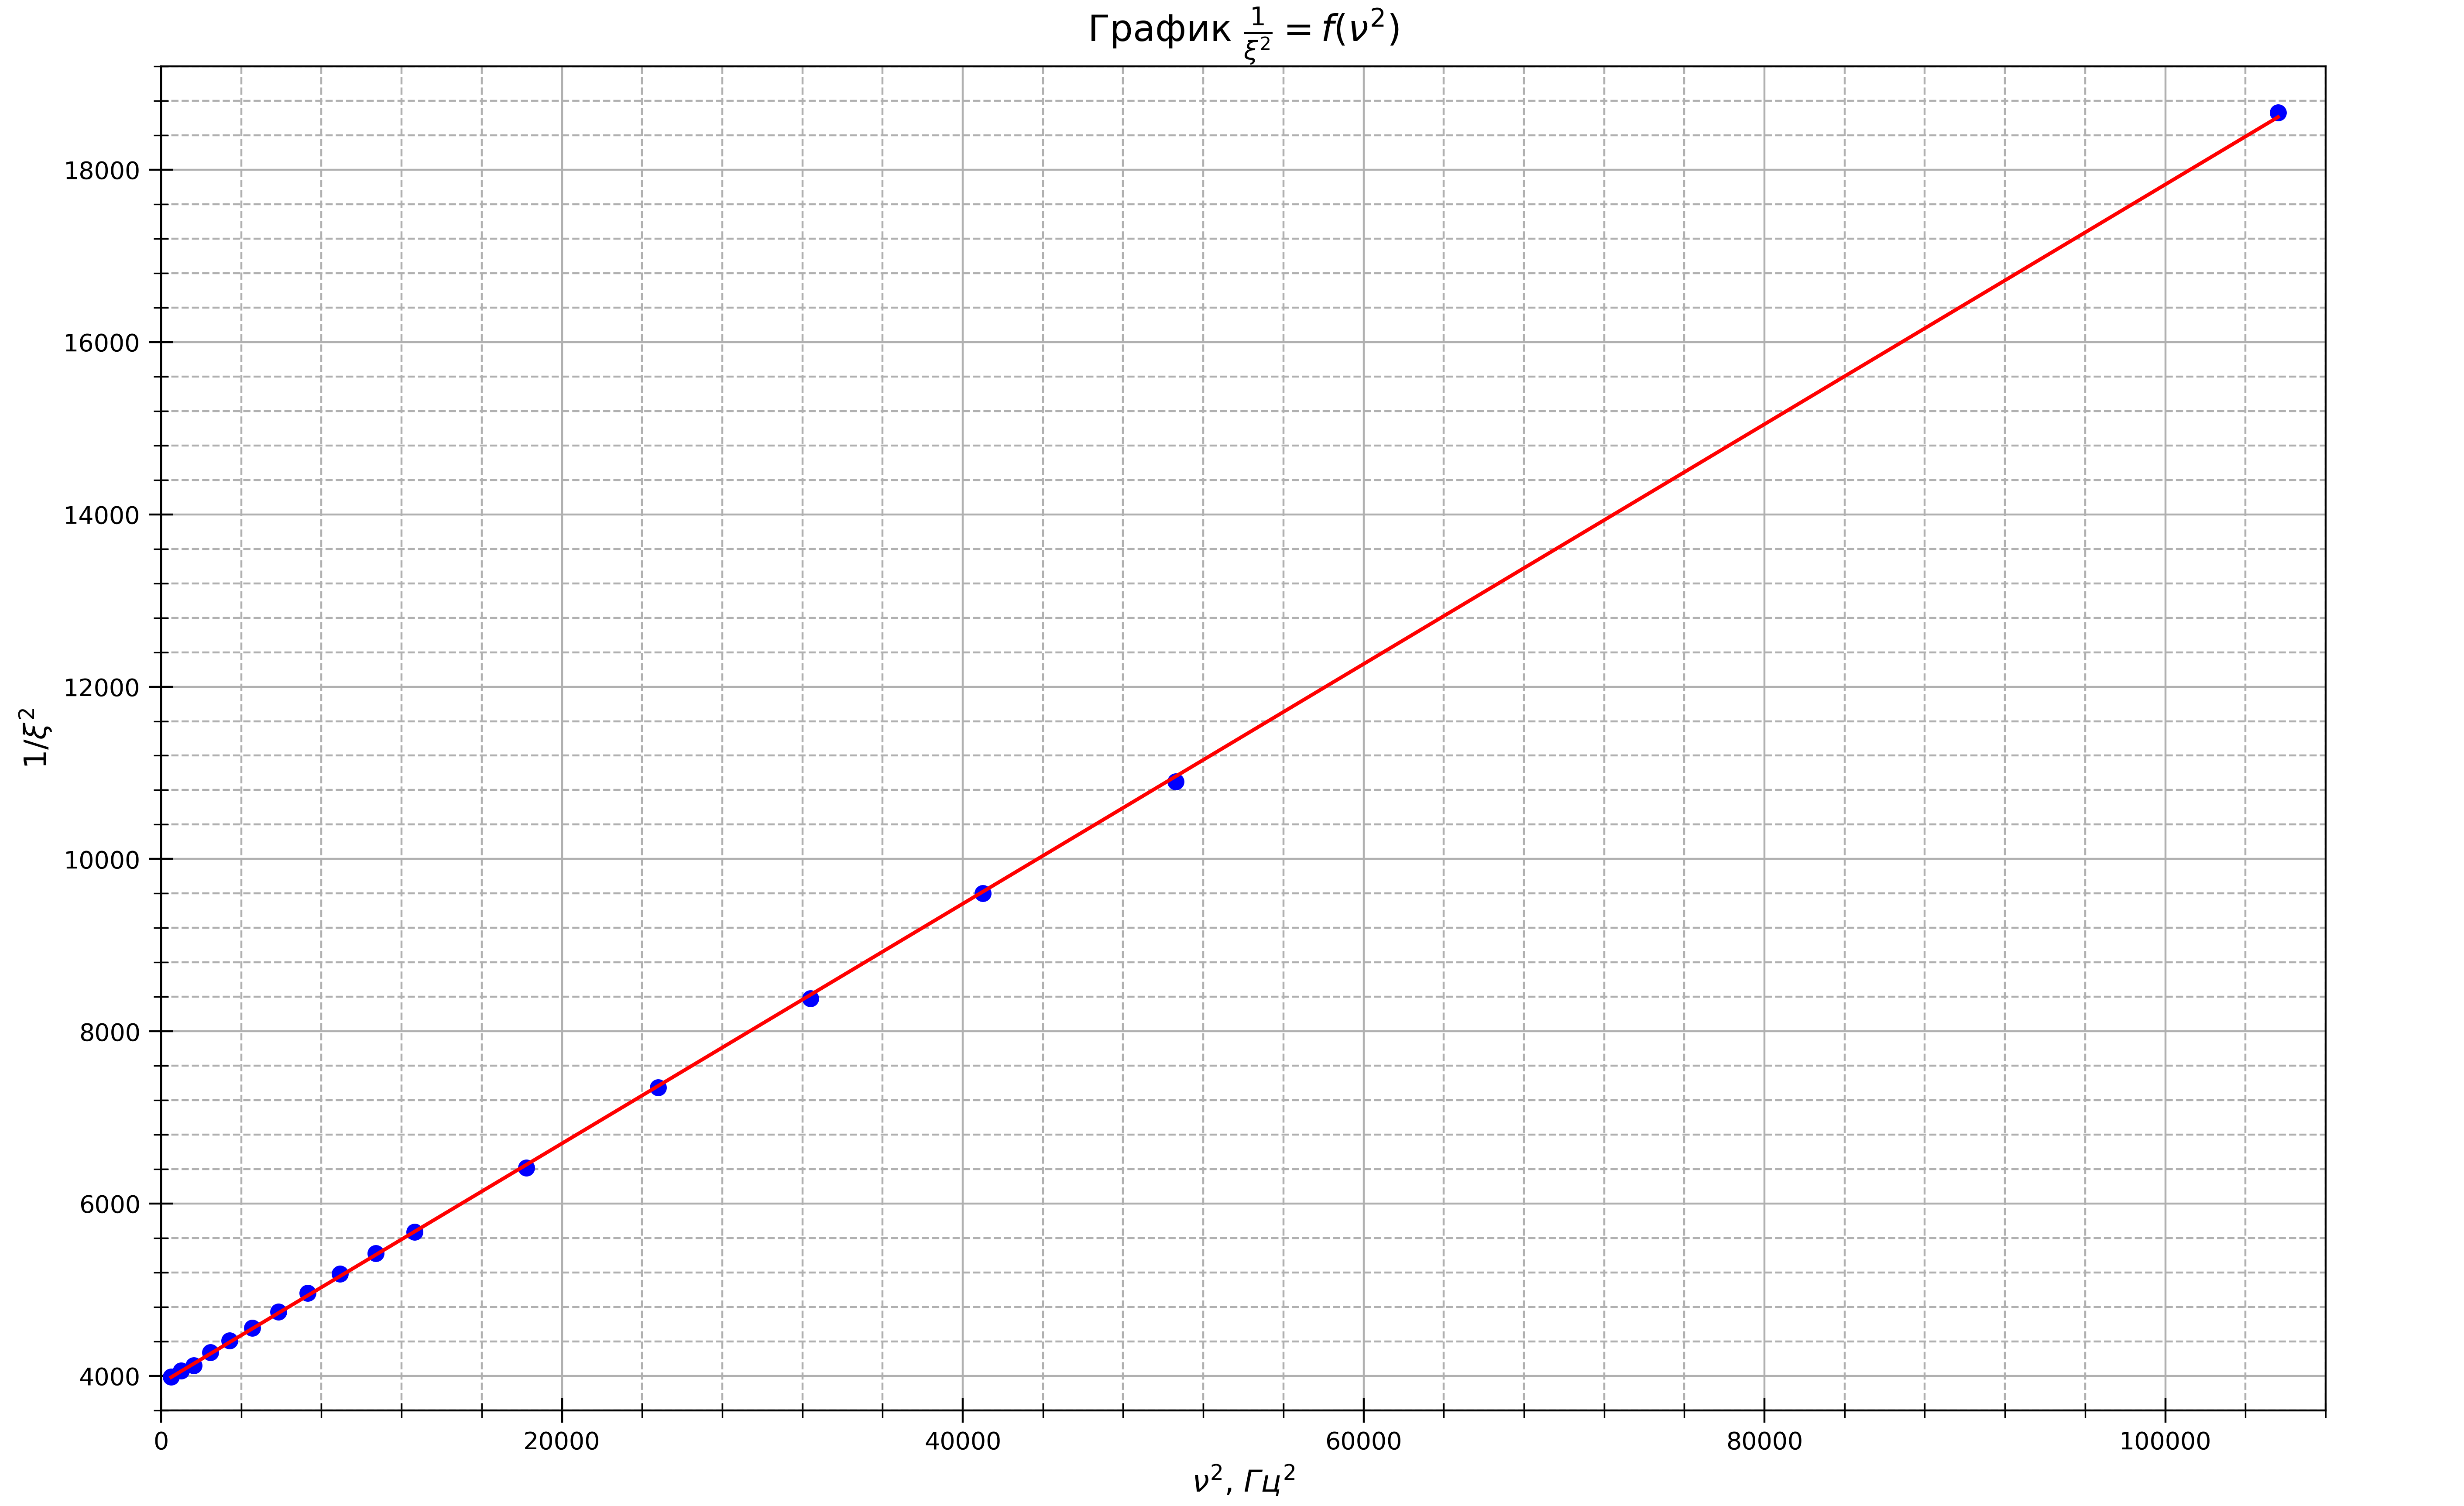
\includegraphics[width=0.9\linewidth]{graph1.png}
\caption{График $\frac{1}{\xi^{2}} = f(\nu^2)$}
\label{fig:mpr}
\end{figure}

При подсчёте получаем $\sigma_1 = (4,20\pm 0,02)\cdot 10^7~\frac{См}{м}$.
\subparagraph{2.} 
Построим график зависимости фазового сдвига от частоты в координатах $tan~\psi(\nu)$. Черех точку ($\psi = \pi/4, \nu = 0$) проведём прямую, которая будет касаться экспериментальной кривой при больших частотах. По наклону этой прямой вычислим значение проводимости меди. Учтём, что присутствует дополнительный свдиг фаз $\frac{\pi}{2}$.
\begin{equation}
    tan~\psi =\frac{ah}{\delta^2}=\frac{1}{2}ah\sigma \mu_0 \omega
\end{equation}
\newpage
\begin{figure}[!h]
\centering
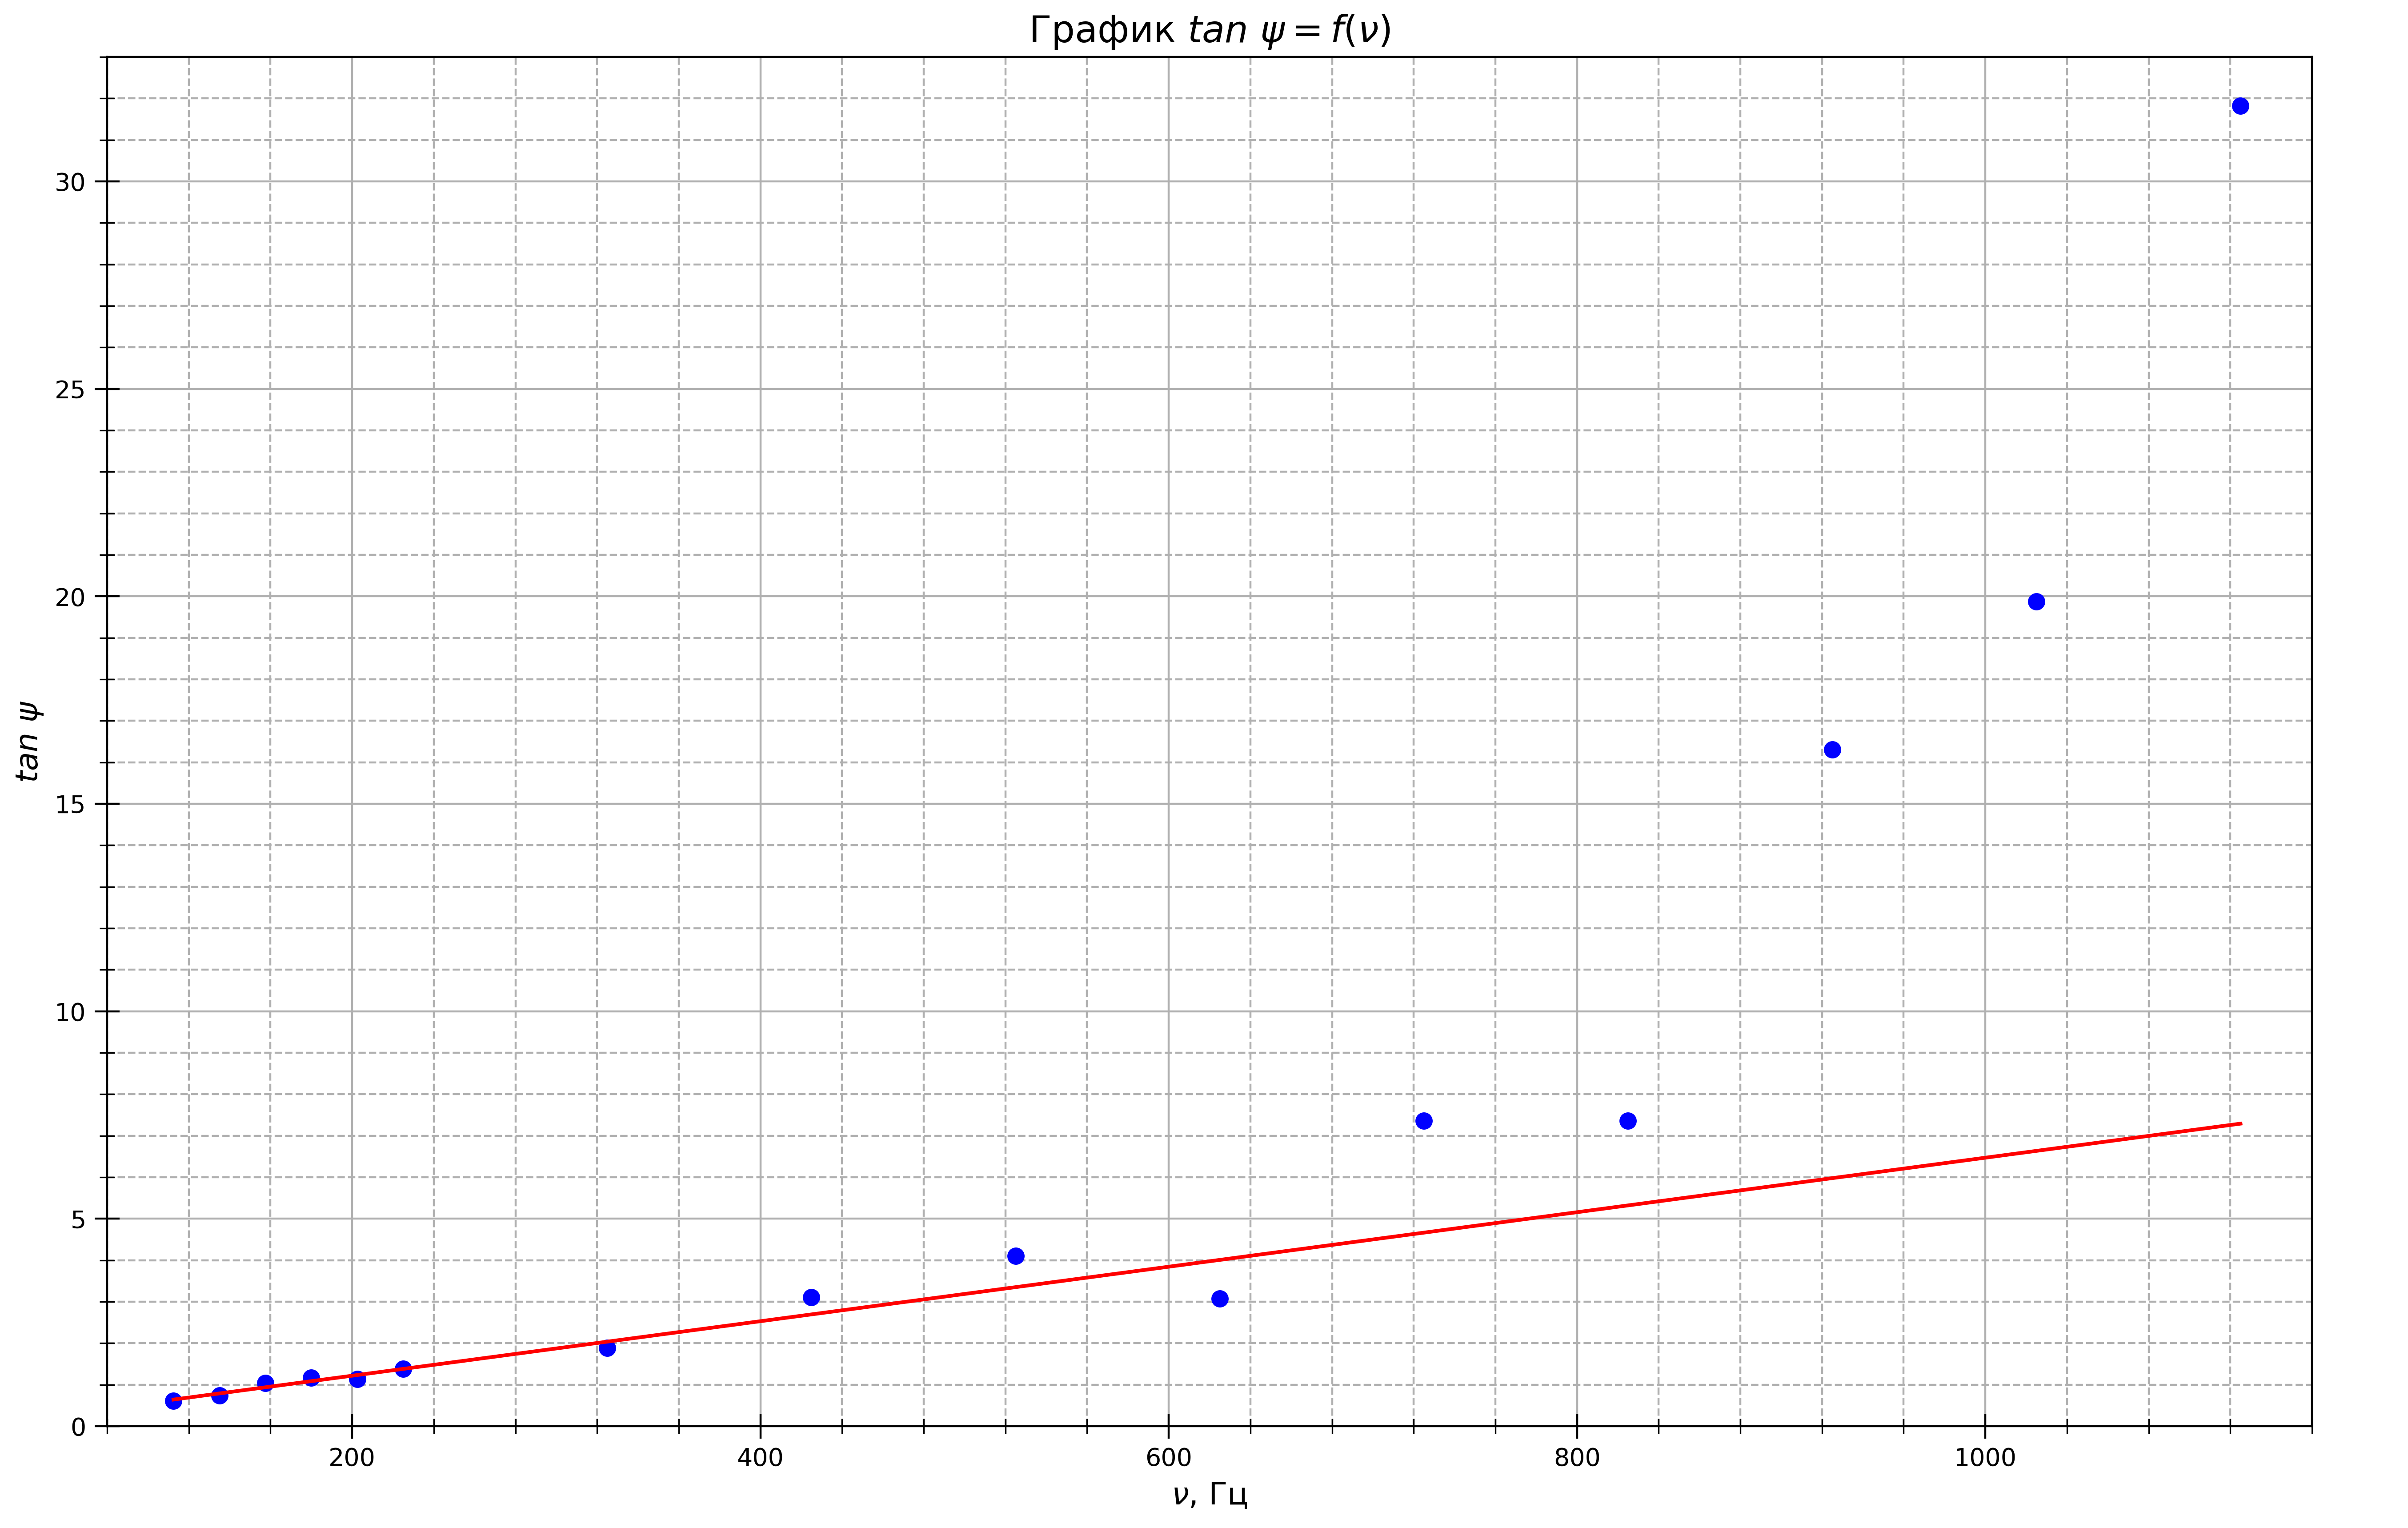
\includegraphics[width=0.9\linewidth]{graph2.png}
\caption{График $tan ~ \psi = f(\nu)$}
\label{fig:mpr}
\end{figure}
Проводимость получается $\sigma_2 = 4,92 \cdot 10^7 ~\frac{См}{м}$.
\subparagraph{3.} Построим график $\psi - \frac{\pi}{4}=f(\sqrt{\nu})$. Проведём прямую через начало координат, которая будет касаться экспериментальной кривой при больших частотах.
\begin{figure}[!h]
\centering
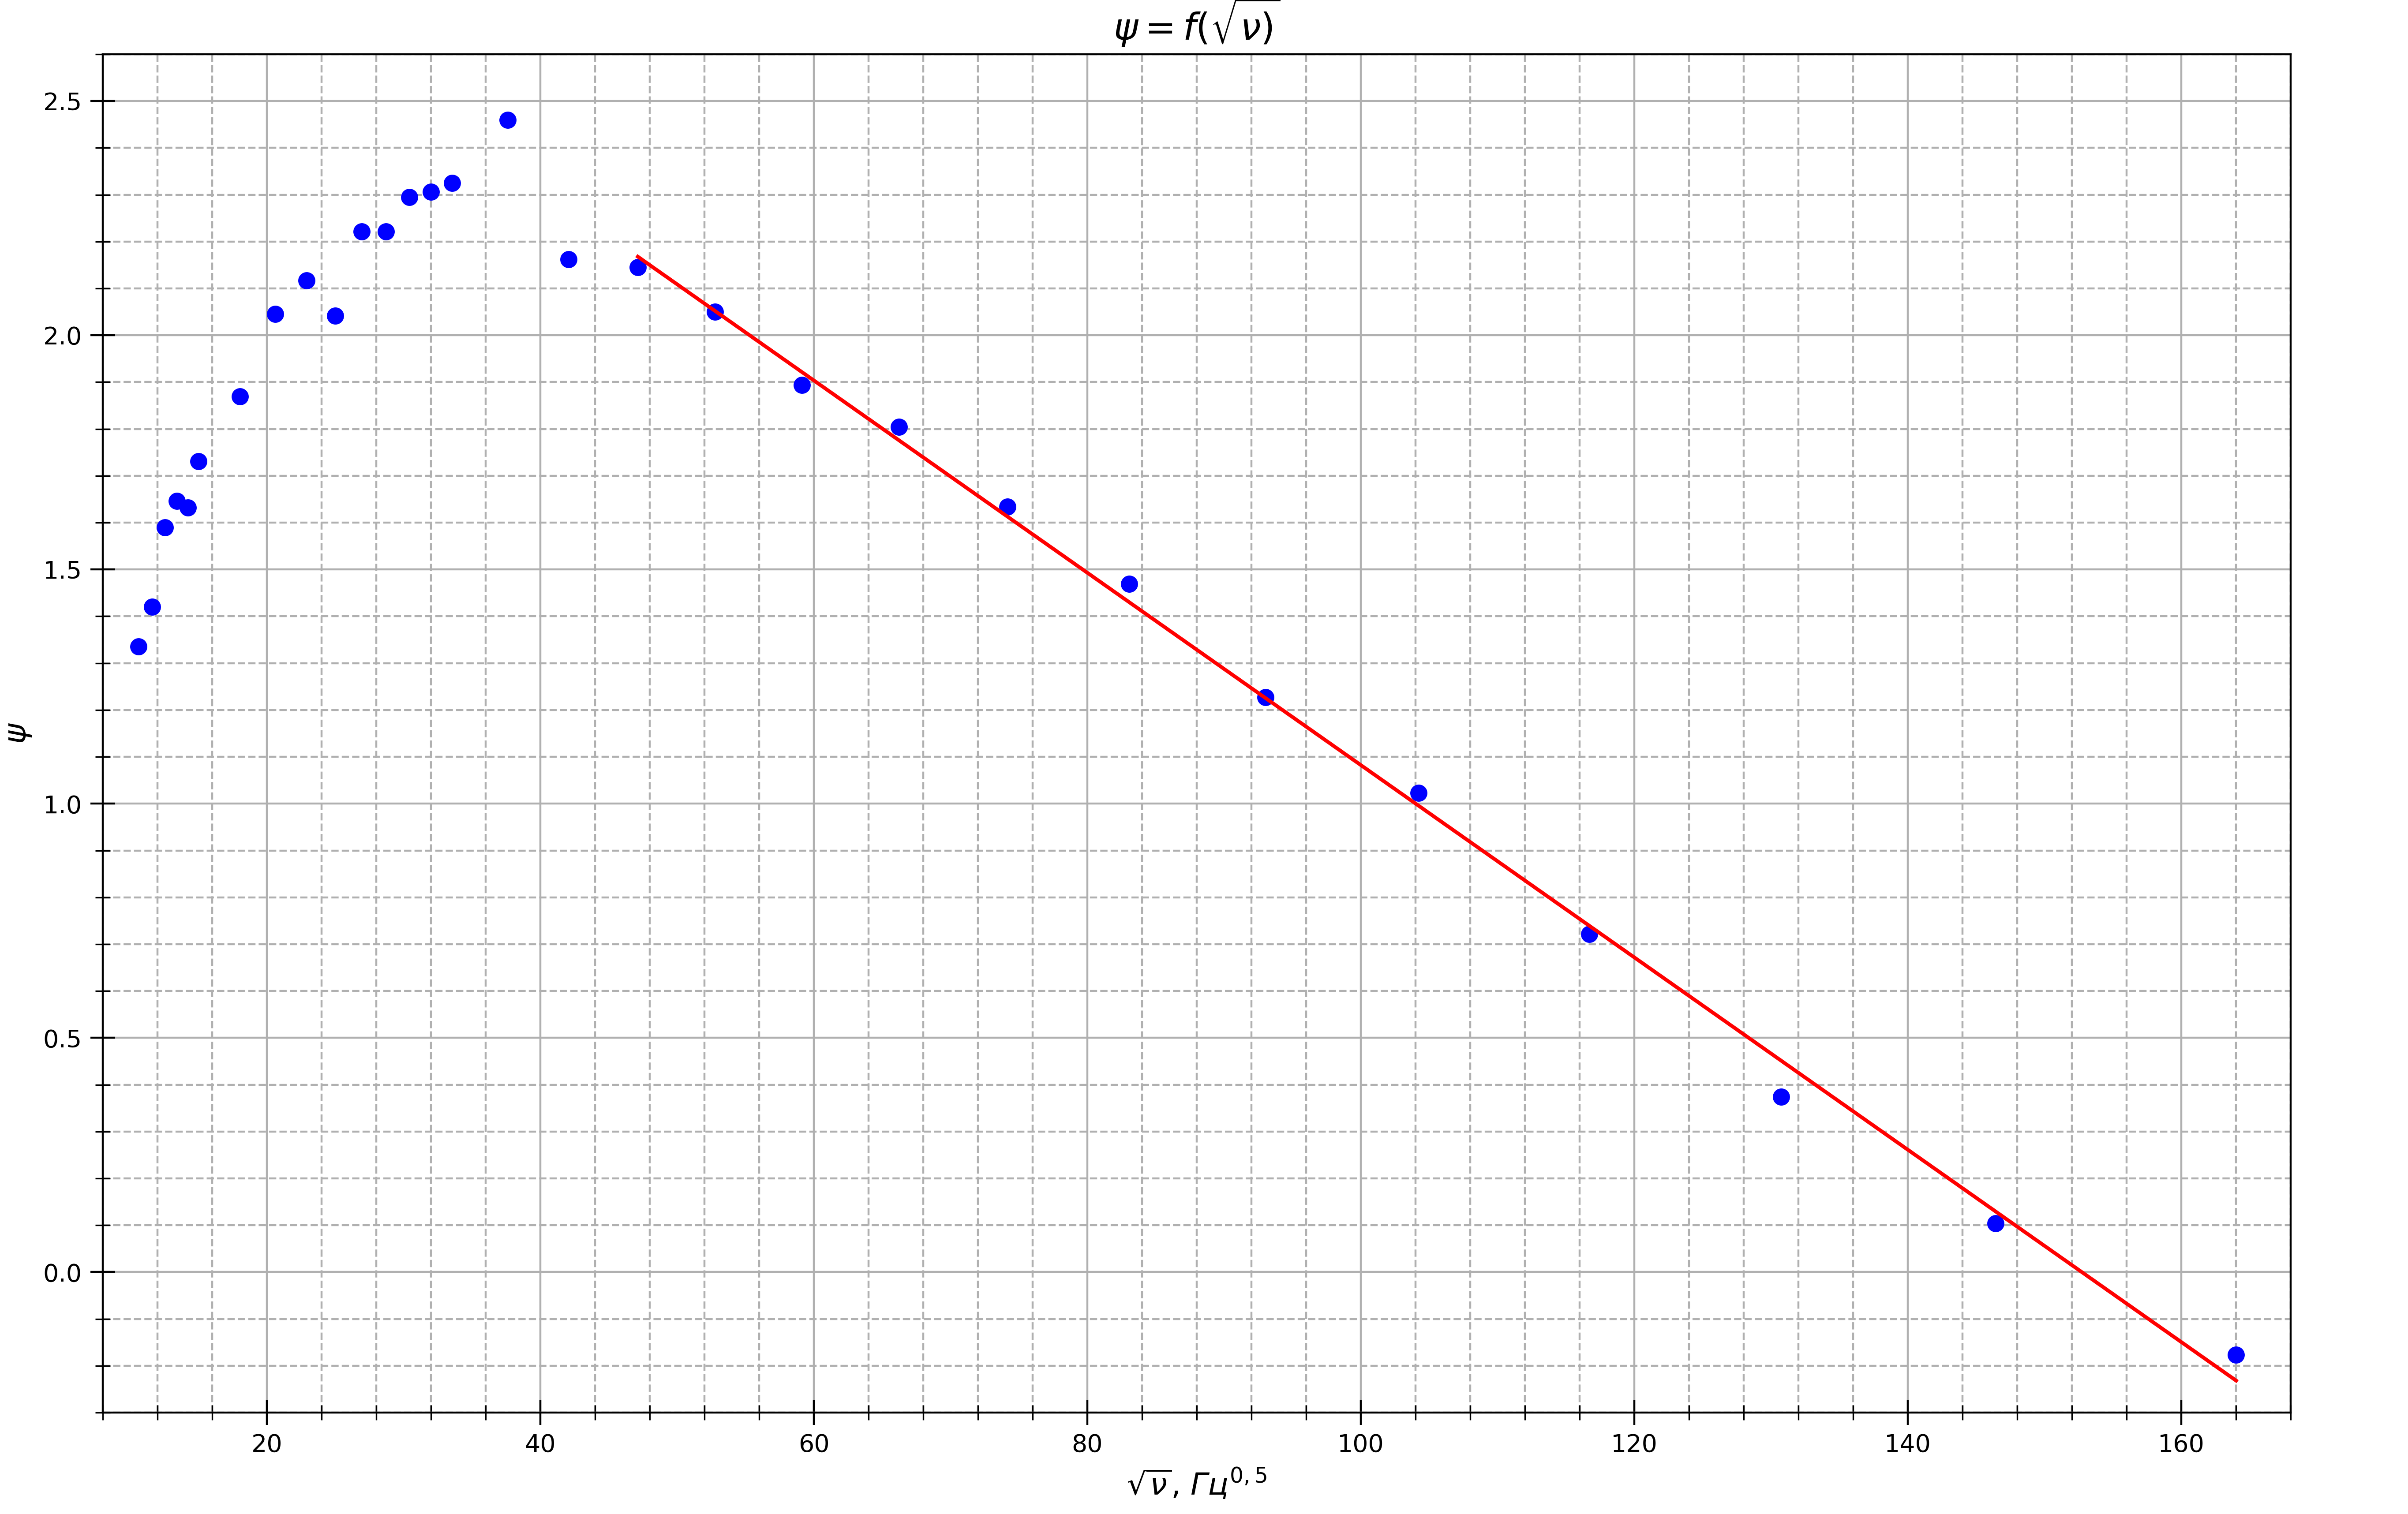
\includegraphics[width=0.9\linewidth]{graph3.png}
\caption{График $\psi = f(\sqrt{\nu})$}
\label{fig:mpr}
\end{figure}
\newpage
Проводимость равна $\sigma_3 = (4,75\pm 0,06)\cdot 10^7~ \frac{См}{м}$.
\subparagraph{4.} Построим график $\frac{L_{max} - L}{L - L_{min}}=f(\nu^2)$. По угловому коэффициенту найдём $\sigma$ меди. $\frac{L_{max} - L}{L - L_{min}}=(\pi ah\mu_0 \sigma \nu)^2$.\par
\begin{figure}[!h]
\centering
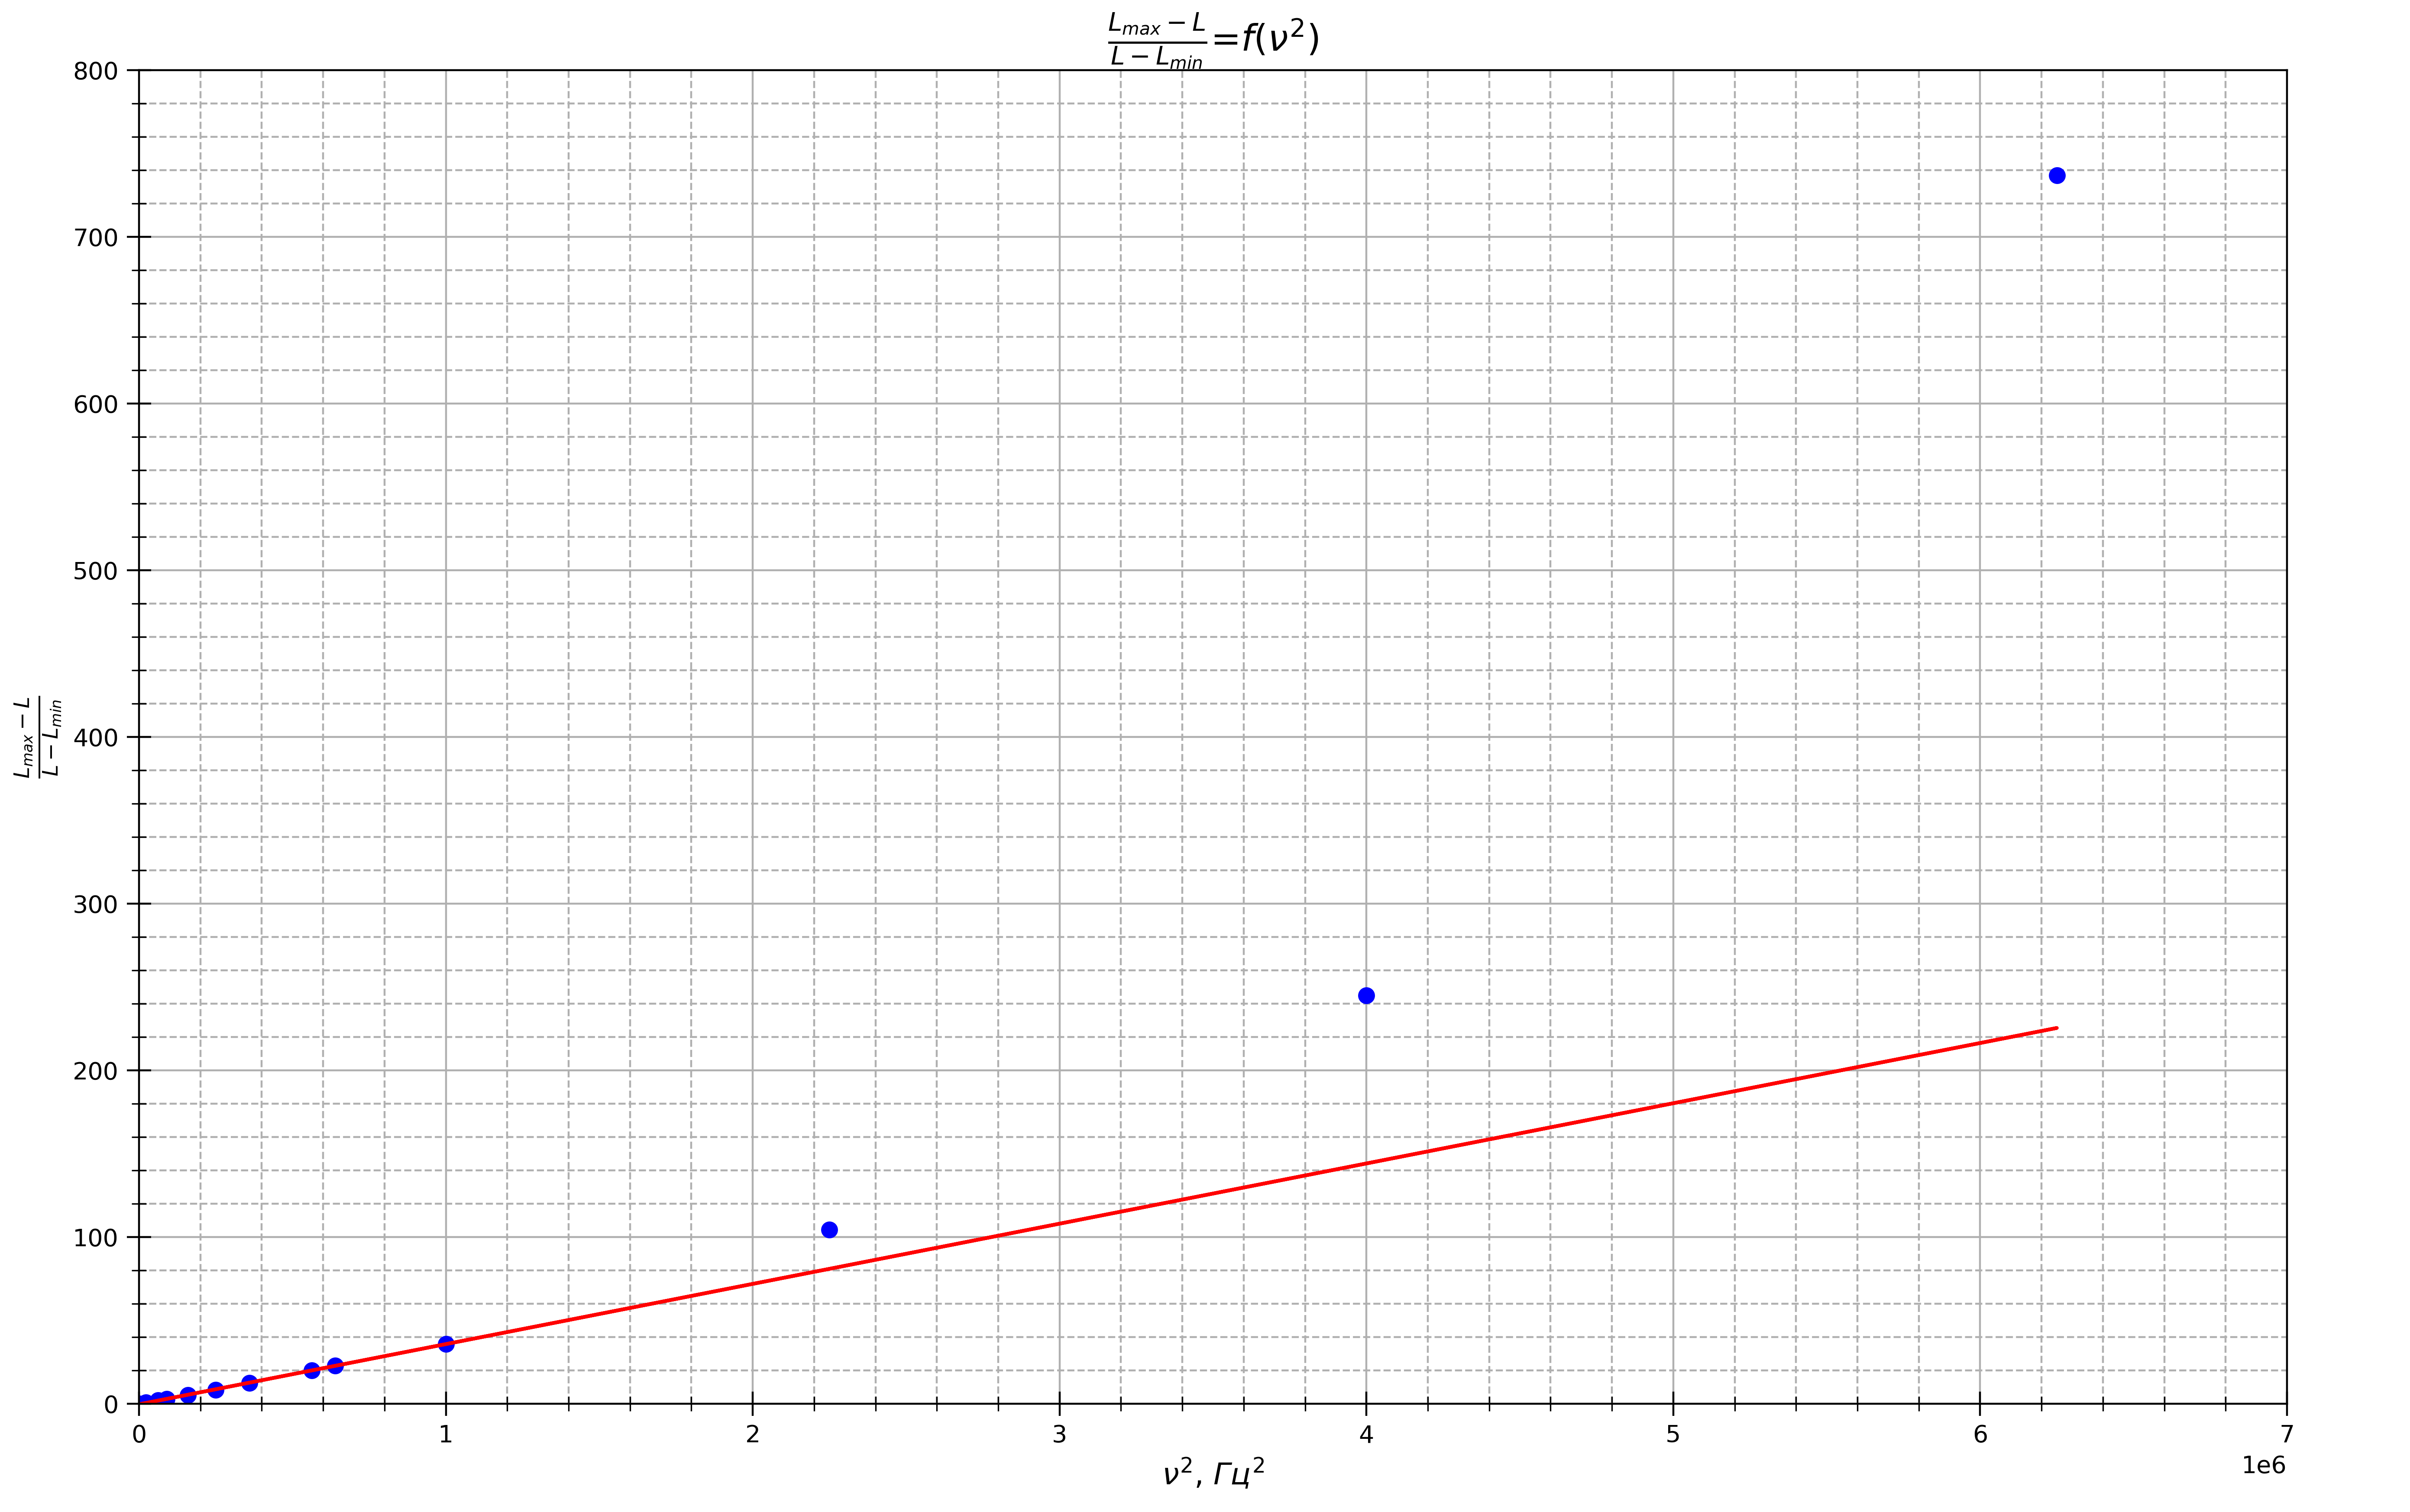
\includegraphics[width=0.9\linewidth]{graph4.png}
\caption{График $\frac{L_{max} - L}{L - L_{min}}=f(\nu^2)$}
\label{fig:mpr}
\end{figure}
Проводимость меди равна $\sigma_4 = (4,51\pm 0,03)\cdot 10^7~ ~\frac{См}{м}$.
\paragraph{Вывод:} в данной лабораторной работе мы исследовали проникновение переменного магнитного поля в медный цилиндр и вычислили проводимость меди с помощью четырёх способов. $\sigma_1 = (4,20\pm 0,02)\cdot 10^7~\frac{См}{м}$, $\sigma_2 = 4,92 \cdot 10^7 ~\frac{См}{м}$, $\sigma_3 = (4,75\pm 0,06)\cdot 10^7~ \frac{См}{м}$, $\sigma_4 = (4,51\pm 0,03)\cdot 10^7~ ~\frac{См}{м}$. Результаты получились близки к табличному значению $\sigma = 5\cdot 10^7 ~\frac{См}{м}$. Наиболее точное значение было найдено вторым способом.
\end{document}
